\documentclass[11pt]{article}

% Change "review" to "final" to generate the final (sometimes called camera-ready) version.
% Change to "preprint" to generate a non-anonymous version with page numbers.
\usepackage[preprint]{acl}

% Standard package includes
\usepackage{times}
\usepackage{latexsym}

% For proper rendering and hyphenation of words containing Latin characters (including in bib files)
\usepackage[T1]{fontenc}
% For Vietnamese characters
% \usepackage[T5]{fontenc}
% See https://www.latex-project.org/help/documentation/encguide.pdf for other character sets

% This assumes your files are encoded as UTF8
\usepackage[utf8]{inputenc}

% This is not strictly necessary, and may be commented out,
% but it will improve the layout of the manuscript,
% and will typically save some space.
\usepackage{microtype}

% This is also not strictly necessary, and may be commented out.
% However, it will improve the aesthetics of text in
% the typewriter font.
\usepackage{inconsolata}

%Including images in your LaTeX document requires adding
%additional package(s)
\usepackage{graphicx}

\usepackage{array}
\usepackage{subcaption} % to have multiple figures in one figure
\usepackage{tabularx} % column width
\usepackage{makecell} % cell size
\usepackage{indentfirst} % indent paragraphs

\graphicspath{ {./images/} }

\title{Project: Medical Question Answering}
\author{Emily Beermann, Ikenna Ojoboh, Ruthresh Pandian, Aman Raj, Shi Qin}


\begin{document}
\maketitle
\begin{abstract}
\end{abstract}

\section{Introduction}
Question answering systems (QAS) are a central goal of Natural Language Processing, aiming to provide precise answers to user input queries in natural language. Such systems can enable efficient access to large-scale information, significantly reducing the time and effort required compared to a manual search. This is particularly relevant in rapidly expanding, highly specialised domains such as biomedical research, where accessing accurate and relevant information can directly influence critical decisions made by clinicians and researchers. As a result, domain-specific QAS provide a useful tool to support evidence-based decision making by facilitating faster and more reliable information retrieval. \par
In our project, we aim to design and implement a QAS capable of answering biomedical questions using the PubMedQA dataset \cite{jin_pubmedqa_2019}. Our primary objective is to investigate how different text representations and model architectures affect the quality of answers. By systematically comparing alternative approaches, we aim to identify which methods are most effective for handling the challenges of biomedical question answering. \par
In order to evaluate variations of our system we use PubMedQA; a dataset constructed from biomedical research papers. Each instance in the dataset consists of a question derived from a research title, a corresponding abstract (excluding the conclusion) that provides context, a long answer (the abstract conclusion), and a yes/no/maybe short answer (Figure \ref{figure:1}). This structure allows the model architecture to be constructed either as classification or as answer generation, allowing for easy comparison of different AI methods. Furthermore, the inputs are provided as paired question-context instances allowing the task to focus on comprehension and reasoning of the text, instead of retrieval, enabling easier evaluation of model performance. \par

% Figure for one intance in PubmedQA dataset
\begin{figure}
\small
\noindent\begin{tabular}{ |m{7cm}| }
\hline
\textbf{Question:} \\ 
Do preoperative statins reduce atrial fibrillation after coronary artery bypass grafting?  \\ 
\textbf{Context:}  \\ 
\textit{(Objective)} Recent studies have demonstrated that statins have pleiotropic effects, including anti-inflammatory effects and atrial fibrillation (AF) preventive effects [...] \newline
\textit{(Methods)} 221 patients underwent CABG in our hospital from 2004 to 2007. 14 patients with preoperative AF and 4 patients with concomitant valve surgery [...] \newline
\textit{(Results)} The overall incidence of postoperative AF was 26\%. Postoperative AF was significantly lower in the Statin group compared with the non-statin group (16\% versus 33\%, p=0.005). Multivariate analysis demonstrated that independent predictors of AF [...] \\
\textbf{Long Answer:} \\
\textit{(Conclusion)} Our study indicated that preoperative statin therapy seems to reduce AF development after CABG. \\
\textbf{Answer:} \\
Yes \\
\hline
\end{tabular}
\caption{An instance \cite{sakamoto_preoperative_2011} from PubMedQA dataset \cite{jin_pubmedqa_2019}.}
\label{figure:1}
\end{figure}

However, biomedical data can provide significant challenges. The language in research papers often contains complex terminology, domain-specific phrases and abbreviations which can be difficult for models to interpret. Additionally, abstracts are usually dense and information-rich, requiring models to identify and extract relevant details from long passages of text. This is highlighted by Figure \ref{figure:subim1} which demonstrates an average context length of 1350 words and some contexts exceeding 2500 words. Many questions also require inferential reasoning rather than simple keyword matching, further increasing difficulty. Our dataset demonstrates a significant label imbalance with 55.2\% of instances belonging in the ‘yes’ class, 33.8\% in the ‘no’ class and only 11\% in the ‘maybe’ class (Figure \ref{figure:subim3}). This distribution indicates that accuracy alone will be an insufficient metric and inspecting macro-average F1 will be required to better understand model performance. These challenges highlight the importance of selecting appropriate text representations and architecture in order to achieve high accuracy and reliability. \par

% EDA Figure
\begin{figure}[h]
\centering
% Question + Context length distribution
\begin{subfigure}{0.9\columnwidth}
\centering
\caption{Context Length Distribution}
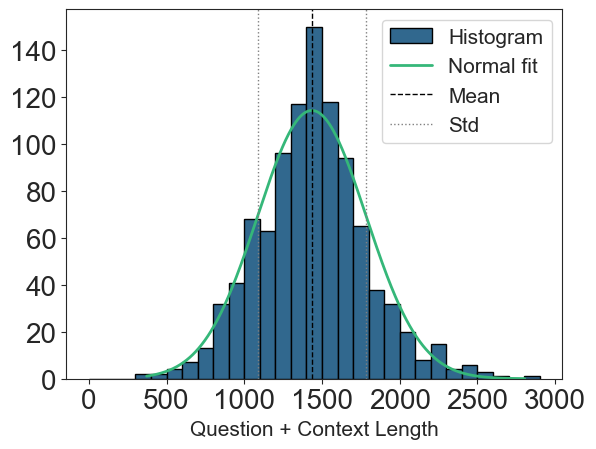
\includegraphics[width=0.9\linewidth, height=5cm]{question_context_hist} 
\label{figure:subim1}
\end{subfigure}
% Label distribution
\begin{subfigure}{0.9\columnwidth}
\centering
\caption{Label Distribution}
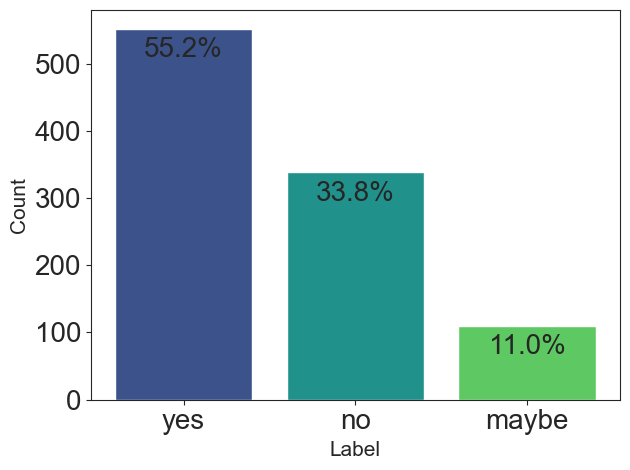
\includegraphics[width=0.9\linewidth, height=5cm]{label_dist}
\label{figure:subim2}
\end{subfigure}
\caption{Data Exploration}
\label{figure:2}
\end{figure}

A key factor influencing QAS performance is text representation. Traditional bag-of-words and TF-IDF representations are simple and easy to interpret but often fail to capture semantic relationships and contextual meaning. In contrast, more advanced embedding-based-methods can represent text in a way that better captures meaning and context which is particularly important in specialised domains. A further key design consideration is model selection. Classification approaches are typically more efficient, and performance is easier to evaluate, especially when answers are limited to predetermined labels. However, they may struggle to capture nuance. In comparison, generative models are more flexible and can produce stronger answer but provide additional challenges such as increased complexity and potential for error. Understanding how text presentation and model architecture interact to affect answer quality is key to optimising performance. \par
A good solution will be able to accurately interpret both the question and context, understand domain-specific semantics, and produce answers that are reliable and consistent.  This project evaluates how different text representations and machine learning methods influence the performance of a biomedical QAS by assessing answer quality. \par


\section{Methods}

\subsection{Baseline System}
The baseline system (Figure \ref{figure:3}) follows a pipeline of six stages. The input, consisting of a question paired with a corresponding abstract, undergoes preprocessing which is handled implicitly by the vectorization step. The processed text is transformed into sparse feature vectors using TF-IDF, capturing term importance. Text representations are then passed into the model, a logistic regression classifier which predicts the most probable answer label. Finally, the system is evaluated using accuracy and F1-score to measure model performance.

% Baseline System Figure
\begin{figure}
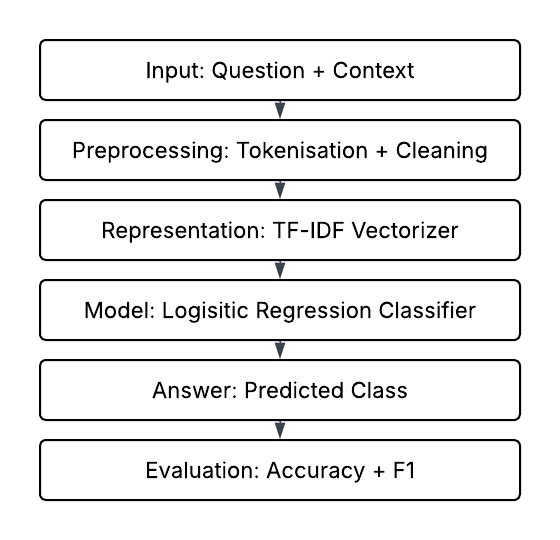
\includegraphics[width=0.9\linewidth, height=6cm]{Baseline} 
\caption{Baseline System}
\label{figure:3}
\end{figure}

\subsection{Axes of Experimentation}
In order to evaluate performance and answer quality we systematically experiment with variations in text representation and AI method. We compare sparse text representations with denser embeddings and compare classification methods to answer generation. These two components are most influential in overall system performance and improvements in these components is expected to provide significant performance gains. Text representation choice determines how effectively meaningful information is captured from the input, while the model choice dictates how that information can be used to make accurate predictions.  Additionally, the two components are interdependent, as different AI methods require different forms of input data so modifying the model necessitates corresponding changes in the input text representation. We therefore evaluate a set of representative pairings that align with the requirements of each method (Figure \ref{table:1}). 

% Alternative Table of Pairings
%\begin{figure}
%\noindent\begin{tabular}{ |m{7cm}| }
%\hline
%\textbf{Experiment 0 (Baseline):} \\ 
%TF-IDF + Logistic Regression \\ 
%\textbf{Experiment 1:} \\ 
%BiomedBERT + Logistic Regression \\ 
%\textbf{Experiment 2:} \\ 
%BioClinical ModernBERT + Logistic Regression/Multilayer Perceptron \\
%\textbf{Experiment 3:} \\ 
%Raw text + BioGPT-Large \\ 
%\textbf{Experiment 4:} \\ 
%Raw text + BioGPT-Large with BioMed-R1-8B \\ 
%\hline
%\end{tabular}
%\caption{Experimental Setup showing text representation and model pairings across baseline and four experiments.}
%\label{figure:4}
%\end{figure}

% Table of Pairings
\begin{table}[htbp]
\centering
\renewcommand{\arraystretch}{1.5}
\begin{tabularx}{\columnwidth}{|l|X|X|}
\hline
& \makecell{\textbf{Text}\\\textbf{Representation}} & \makecell{\textbf{Model}}\\
\hline
\textbf{Baseline} & \makecell{TF-IDF} & \makecell{Logistic\\Regression} \\
\hline
\textbf{Exp 1} & \makecell{BiomedBERT} & \makecell{Logistic\\Regression} \\
\hline
\textbf{Exp 2} & \makecell{BioClinical\\ModernBERT} & \makecell{Logistic\\Regression} \\
\hline
\textbf{Exp 3} & \makecell{Raw text} & \makecell{BioGPT} \\
\hline
\textbf{Exp 4} & \makecell{Raw text} & \makecell{BioMed-R1-8B} \\
\hline
\end{tabularx}
\caption{Experimental Pairings}
\label{table:1}
\end{table}


\subsection{Proposed Improvements}
Text representation a key component of the pipeline as it determines how linguistic and semantic information is captured from the input. Models must reason over long, information-dense contexts which will be particularly challenging for sparse representations. The baseline system, using TF-IDF text representation is expected to perform adequately on straightforward instances but will struggle with complex questions and abstracts. TF-IDF representations are not able to capture word order and context which limits their ability to capture nuanced meanings and semantic relationships between words. We compare our baseline system using sparse text representation to BERT-based contextual embeddings. Contextual embeddings generated by pretrained biomedical language models BiomedBERT and BioClinical ModernBERT are able to encapsulate context-dependant meanings and are therefore expected to perform better. Multi-phase fine-tuning of BioBERT with long-answer bag-of-word statistics as additional supervision has previously achieved 68.1\% accuracy \cite{jin_pubmedqa_2019}. However this is significantly lower than single-human performance of 78\% accuracy (Figure \ref{table:1}) demonstrating a need for improvement. 
The second key component of our QA pipeline is the AI method. The baseline system uses a logistic regression classifier which is chosen for its simplicity, interpretability and effectiveness on high-dimensional sparse data. While it provides a strong and efficient baseline, its performance is limited by its linear nature. This restricts its ability to capture complex patterns and interactions within the data. To address these limitations we compare our baseline system to two alternative prediction models: multilayer perceptrons (MLPs) and large language models. MLPs are expected to improve performance by enabling the model to capture nonlinear relationships within dense embeddings, allowing for more complex decision boundaries. Large language models are expected to provide the greatest performance gain as they integrate representation learning and reasoning within a single architecture making them better able to handle the complexities of biomedical language. Compared to logistic regression these models can extract and utilise contextual information from the text, resulting in increased performance particularly on more complex questions requiring deeper semantic understanding and inference. 

\begin{table}[htbp]
\centering
\begin{tabular}{|l|c|c|}
\hline
& \textbf{Accuracy} & \textbf{F1} \\
\hline
\makecell{\textbf{Majority}\\\textbf{Performance}} & 0.552000 & 0.237113 \\
\hline
\makecell{\textbf{Reasoning-free}\\\textbf{Human Performance}} & 0.904000 & 0.841823 \\
\hline
\makecell{\textbf{Reasoning-required}\\\textbf{Human Performance}} & 0.780000 & 0.721920 \\
\hline
\end{tabular}
\caption{Human Performance}
\label{table:2}
\end{table}



\section{Experimental Evaluation}

\subsection{Experimental Setup}

\subsection{Results}

\subsection{Error Analysis}

\subsection{Discussion}


\section{Conclusion}


\bibliography{Overleaf_Report/References}


\end{document}
